\documentclass{article}
\usepackage[utf8x]{inputenc}
\usepackage{ucs}
\usepackage{amsmath} 
\usepackage{amsfonts}
\usepackage{upgreek}
\usepackage[english,russian]{babel}
\usepackage{graphicx}
\usepackage{float}
\usepackage{textcomp}
\usepackage{hyperref}
\usepackage{geometry}
  \geometry{left=2cm}
  \geometry{right=1.5cm}
  \geometry{top=1cm}
  \geometry{bottom=2cm}
\usepackage{tikz}
\usepackage{ccaption}
\usepackage{multicol}

\usepackage{listings}
%\setlength{\columnsep}{1.5cm}
%\setlength{\columnseprule}{0.2pt}


\begin{document}
\pagenumbering{gobble}

\lstset{
  language=C,                % choose the language of the code
  basicstyle=\linespread{1.1}\ttfamily,
  columns=fixed,
  fontadjust=true,
  basewidth=0.5em,
  keywordstyle=\color{blue}\bfseries,
  commentstyle=\color{gray},
  stringstyle=\ttfamily\color{orange!50!black},
  showstringspaces=false,
  %numbers=false,                   % where to put the line-numbers
  numbersep=5pt,
  numberstyle=\tiny\color{black},
  numberfirstline=true,
  stepnumber=1,                   % the step between two line-numbers.        
  numbersep=10pt,                  % how far the line-numbers are from the code
  backgroundcolor=\color{white},  % choose the background color. You must add \usepackage{color}
  showstringspaces=false,         % underline spaces within strings
  captionpos=b,                   % sets the caption-position to bottom
  breaklines=true,                % sets automatic line breaking
  breakatwhitespace=true,         % sets if automatic breaks should only happen at whitespace
  xleftmargin=.2in,
  extendedchars=\true,
  keepspaces = true,
}
\lstset{literate=%
   *{0}{{{\color{red!20!violet}0}}}1
    {1}{{{\color{red!20!violet}1}}}1
    {2}{{{\color{red!20!violet}2}}}1
    {3}{{{\color{red!20!violet}3}}}1
    {4}{{{\color{red!20!violet}4}}}1
    {5}{{{\color{red!20!violet}5}}}1
    {6}{{{\color{red!20!violet}6}}}1
    {7}{{{\color{red!20!violet}7}}}1
    {8}{{{\color{red!20!violet}8}}}1
    {9}{{{\color{red!20!violet}9}}}1
}

\title{Семинар \#1: Основы C. Ввод/вывод. Операторы. Циклы. Массивы. \vspace{-5ex}}\date{}\maketitle
\section*{Ввод/вывод}
\subsection*{Hello World!}
Программа на языке C, которая печатает на экран строку \texttt{Hello world} выглядит следующим образом:
\begin{lstlisting}
#include <stdio.h>
int main() 
{
    printf("Hello world\n");
}
\end{lstlisting}


\subsection*{Функции \texttt{printf} и \texttt{scanf}}
\begin{itemize}
\item Функция \texttt{printf} используется для печати на экран всего что угодно.
\item Функция \texttt{scanf} используется для считывания значений переменных с экрана.
\item Обе эти функции хранятся в библиотеке \texttt{stdio.h}. Эту библиотеку нужно подключить с помощью
\begin{lstlisting}
#include <stdio.h>
\end{lstlisting}
\end{itemize}

\subsection*{Целочисленные переменные \texttt{int}:}
\begin{itemize}
\item Переменные типа \texttt{int} нужны для хранения целых чисел.
\end{itemize}


\subsection*{Адрес и размер переменной:}
\begin{itemize}
\item 1 бит - минимальная единица измерения памяти. В 1 бите может хранится либо \texttt{0} либо \texttt{1}.
\item Вся память делится на ячейки, размером в 8 бит = 1 байт.
\item Все эти ячейки занумерованы, номер ячейки называется адресом.
\item Все переменные содержатся в памяти. Адрес переменной - это адрес первого байта переменной.
\item Чтобы найти адрес переменной, нужно перед ней поставить \texttt{\&}, например, \texttt{\&a}
\item Функции \texttt{scanf} нужно передавать именно адрес переменной, а не само значение переменной.
\item Чтобы найти размер переменной в байтах: \texttt{sizeof(a)}
\item Например, переменная типа \texttt{int} имеет размер 4 байта = 32 бита. Значит в ней может хранится максимум $2^{32}$ значений. То есть переменные типа \texttt{int} могут принимать значения от $-2^{31}$ до $2^{31}$.
\end{itemize}

\begin{center}
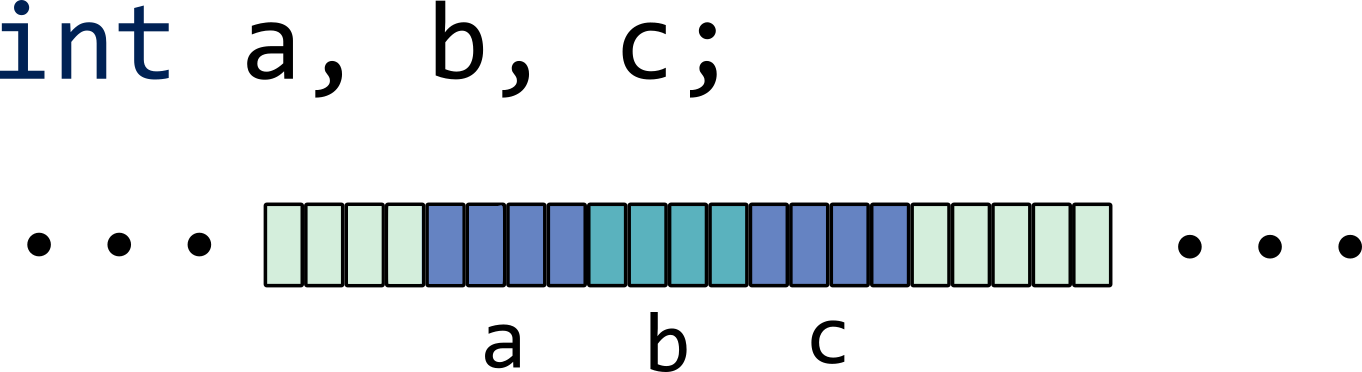
\includegraphics[scale=0.6]{../images/memory_ints.png}
\end{center}

\newpage
\section*{Операторы}

\subsection*{Арифметические операторы и операторы присваивания:}
\texttt{
\begin{multicols}{2}
\begin{tabular}{ c c } 
 + & сложение \\  
 - & вычитание \\  
 * & умножение \\ 
 / & целочисленное деление \\
 \% & остаток \\
\end{tabular}
\vfill
\begin{tabular}{ c c }
 = & присвоить левой части правую\\ 
 += & прибавить к левой части правую \\  
 -= & отнять от левой части правую \\  
 /= & разделить левую часть на правую \\ 
 \%= & левая часть становится равна остатку\\
 ++  & увеличить на 1\\
 -{}-  & уменьшить на 1
\end{tabular}
\end{multicols}
}

\subsection*{Операторы сравнения и логические операторы:}
\begin{center}
\texttt{
\begin{multicols}{2}
\begin{tabular}{ c c }
 == & равно\\ 
 != & не равно \\  
 > & больше \\  
 >= & больше или равно \\ 
 < & меньше \\
 <= & меньше или равно \\
\end{tabular}
\vfill
\begin{tabular}{ c c }
 \&\& & логическое И \\ 
 || & логическое ИЛИ \\  
 !  & логическое НЕ \\  
\end{tabular}
\end{multicols}
}
\end{center}


\subsection*{Условный оператор:}
\begin{center}
\begin{lstlisting}
                                     if ( условие1 )
                                         сделай это
                                     else if ( условие2 )
                                     	 сделай это
                                     else
                                         сделай это
\end{lstlisting}
\end{center}


\section*{Циклы}

\subsection*{Цикл \texttt{while}:}
\begin{lstlisting}
                                     while ( условие )
                                     {
                                         делай это
                                     }
\end{lstlisting}

\subsection*{Цикл \texttt{for}:}
Циклом \texttt{for} обычно удобнее пользоваться. Соответствие между циклами \texttt{while} и \texttt{for}: \\

\begin{lstlisting}
            инициализация
            while ( условие )                    for ( инициализация; условие; обновление )
            {                                    {        
                делай это             -->            делай это                       
                обновление                       }                     
            }                                                
\end{lstlisting}


\section*{Массивы}
Массивы - это объекты, которые могут хранить внутри себя большое количество других объектов одного типа.
Например, мы можем создать массив, который будет хранить 6 чисел типа \texttt{int} вот так:

\lstset{
  xleftmargin=.3\textwidth, xrightmargin=.2\textwidth
}
\begin{lstlisting}
int a[6] = {4, 8, 15, 16, 23, 42};
\end{lstlisting}

После того, как мы создали массив, мы можем получать доступ к каждому элементу массива по номеру. Номер
элемента массива также называется его индексом. При этом нумерация в массиве начинается с нуля.
\begin{center}
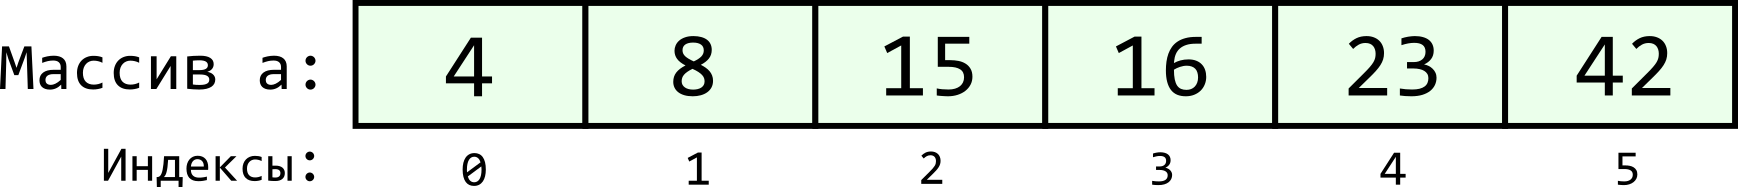
\includegraphics[scale=0.8]{../images/array_indexes.png}
\end{center}
Доступ к элементу по индексу осуществляется через квадратные скобки. Например, если мы хотим поменять в массиве, определённом выше, число 15 на 20 нужно написать:
\begin{lstlisting}
a[2] = 20;
\end{lstlisting}



\subsection*{Подмассивы}
Подмассив - это некоторая последовательная часть массива. В языке C нет никаких специальных средств для работы с подмассивами. Мы будем задавать подмассив в коде как два числа -- индексы граничных элементов. Будем обозначать подмассивом \texttt{a[l, r]} такую часть массива, элементы которого имеют индекс \texttt{i} в диапазоне \\
\texttt{l <= i < r}. Обратите внимание, что мы договорились, что элемент \texttt{a[r]} не входит в подмассив \texttt{a[l, r]}.\\

Например, в подмассив \texttt{[1, 4]} массива \texttt{a} входят элементы \texttt{8, 15, 16}, а элемент \texttt{23} не входит.
\begin{center}
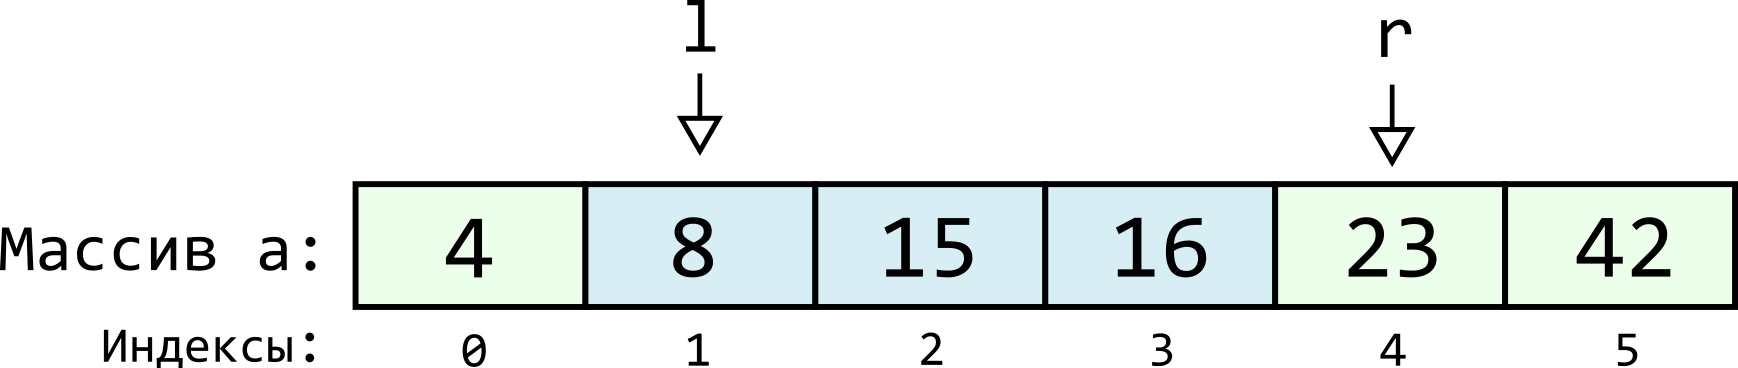
\includegraphics[scale=0.8]{../images/array_slice.png}
\end{center}


\subsection*{Сортировка}
Сортировка -- это упорядочение элементов по возрастанию, убыванию или по какому-то другому критерию.

\subsubsection*{Сортировка выбором} 
Сортировка выбором -- это простейший алгоритм сортировки, который заключается в следующем: \\
Для каждого подмассива \texttt{[j, n]} (где \texttt{j} последовательно меняется от \texttt{0} до \texttt{n - 1}) поменять местами первый и минимальный элементы этого подмассива. 


\begin{lstlisting}
for (int j = 0; j < n; ++j)
{
    int min_index = j;
    for (int i = j + 1; i < n; ++i)
    {
        if (a[i] < a[min_index])
            min_index = i;
    }

    int temp = a[j];
    a[j] = a[min_index];
    a[min_index] = temp;
}
\end{lstlisting}

\subsubsection*{Сортировка пузырьком} 
Сортировка пузырьком -- это простейший алгоритм сортировки, который заключается в следующем: \\
Для каждого подмассива \texttt{[0, n - j]} (где \texttt{j} последовательно меняется от \texttt{0} до \texttt{n - 1}) мы делаем следующую операцию: пробегаем по этому подмассиву и, если соседние элементы стоят неправильно, то меняем их местами.


\begin{lstlisting}
for (int j = 0; j < n; ++j)
{
    for (int i = 0; i < n - 1 - j; i += 1)
    {
        if (a[i] > a[i + 1])
        {
            int temp = a[i];
            a[i] = a[i + 1];
            a[i + 1] = temp;
        }
    }
}
\end{lstlisting}


\subsection*{Бинарный поиск на отсортированном массиве}
Если известно, что массив уже отсортирован, то многие задачи на таком массиве можно решить гораздо проще и/или эффективней. Например, просто найти минимум, максимум и медианное значение. Одной из задач, которая быстрее решается на отсортированном массиве -- это задача поиска элемента в массиве. Если массив отсортирован, то решить эту задачу можно гораздо быстрее чем простой обход всех элементов. \\

Предположим, что массив отсортирован по возрастанию и надо найти элемент \texttt{x} в этом массиве или понять, что такого элемента в массиве не существует. Для этого мы мысленно разделим массив на  2 части:
\begin{enumerate}
\item Элементы, которые меньше, чем \texttt{x}
\item Элементы, которые больше или равны \texttt{x}
\end{enumerate}

Затем введём две переменные-индекса \texttt{l} и \texttt{r}. В начале работы алгоритма индекс \texttt{l} будет хранить индекс фиктивного элемента, находящегося до первого (то есть \texttt{l = -1}), а индекс \texttt{r} будет хранить индекс фиктивного элемента, находящимся после последнего (то есть \texttt{r = n}). 

На каждом шаге алгоритма мы будем брать середину между индексами \texttt{l} и \texttt{r} и передвигать к этой середине или индекс \texttt{l} или индекс \texttt{r}. При этом при изменении индексов должны соблюдаться условия:
\begin{verbatim}
a[l] < x
a[r] >= x
\end{verbatim}

Алгоритм закончится тогда, когда разница между индексами не станет равным 1, то есть не станет \\
\texttt{r == l + 1}. И так как \texttt{a[l] < x} и \texttt{a[r] >= x}, то если элемент \texttt{x} в массиве существует, то его индекс равен \texttt{r}.



Код для поиска в отсортированном массиве бинарным поиском:
\begin{lstlisting}
#include <stdio.h>

int main() 
{
    int n;
    int a[1000];
    scanf("%i", &n);
    for (int i = 0; i < n; ++i)
        scanf("%i", &a[i]);
        
    int x;
    scanf("%i", &x);
    
    int l = -1, r = n;
    while (r > l + 1) 
    {
        int mid = (l + r) / 2;
        
        if (a[mid] >= x)
            r = mid;
        else 
            l = mid;
    }
    
    if (r < n && a[r] == x)
        printf("Element found! Index = %i\n", r);
    else
        printf("Element not found!");
}

\end{lstlisting}

\end{document}